% Options for packages loaded elsewhere
% Options for packages loaded elsewhere
\PassOptionsToPackage{unicode}{hyperref}
\PassOptionsToPackage{hyphens}{url}
\PassOptionsToPackage{dvipsnames,svgnames,x11names}{xcolor}
%
\documentclass[
  letterpaper,
  DIV=11,
  numbers=noendperiod]{scrartcl}
\usepackage{xcolor}
\usepackage{amsmath,amssymb}
\setcounter{secnumdepth}{5}
\usepackage{iftex}
\ifPDFTeX
  \usepackage[T1]{fontenc}
  \usepackage[utf8]{inputenc}
  \usepackage{textcomp} % provide euro and other symbols
\else % if luatex or xetex
  \usepackage{unicode-math} % this also loads fontspec
  \defaultfontfeatures{Scale=MatchLowercase}
  \defaultfontfeatures[\rmfamily]{Ligatures=TeX,Scale=1}
\fi
\usepackage{lmodern}
\ifPDFTeX\else
  % xetex/luatex font selection
\fi
% Use upquote if available, for straight quotes in verbatim environments
\IfFileExists{upquote.sty}{\usepackage{upquote}}{}
\IfFileExists{microtype.sty}{% use microtype if available
  \usepackage[]{microtype}
  \UseMicrotypeSet[protrusion]{basicmath} % disable protrusion for tt fonts
}{}
\makeatletter
\@ifundefined{KOMAClassName}{% if non-KOMA class
  \IfFileExists{parskip.sty}{%
    \usepackage{parskip}
  }{% else
    \setlength{\parindent}{0pt}
    \setlength{\parskip}{6pt plus 2pt minus 1pt}}
}{% if KOMA class
  \KOMAoptions{parskip=half}}
\makeatother
% Make \paragraph and \subparagraph free-standing
\makeatletter
\ifx\paragraph\undefined\else
  \let\oldparagraph\paragraph
  \renewcommand{\paragraph}{
    \@ifstar
      \xxxParagraphStar
      \xxxParagraphNoStar
  }
  \newcommand{\xxxParagraphStar}[1]{\oldparagraph*{#1}\mbox{}}
  \newcommand{\xxxParagraphNoStar}[1]{\oldparagraph{#1}\mbox{}}
\fi
\ifx\subparagraph\undefined\else
  \let\oldsubparagraph\subparagraph
  \renewcommand{\subparagraph}{
    \@ifstar
      \xxxSubParagraphStar
      \xxxSubParagraphNoStar
  }
  \newcommand{\xxxSubParagraphStar}[1]{\oldsubparagraph*{#1}\mbox{}}
  \newcommand{\xxxSubParagraphNoStar}[1]{\oldsubparagraph{#1}\mbox{}}
\fi
\makeatother


\usepackage{longtable,booktabs,array}
\newcounter{none} % for unnumbered tables
\usepackage{calc} % for calculating minipage widths
% Correct order of tables after \paragraph or \subparagraph
\usepackage{etoolbox}
\makeatletter
\patchcmd\longtable{\par}{\if@noskipsec\mbox{}\fi\par}{}{}
\makeatother
% Allow footnotes in longtable head/foot
\IfFileExists{footnotehyper.sty}{\usepackage{footnotehyper}}{\usepackage{footnote}}
\makesavenoteenv{longtable}
\usepackage{graphicx}
\makeatletter
\newsavebox\pandoc@box
\newcommand*\pandocbounded[1]{% scales image to fit in text height/width
  \sbox\pandoc@box{#1}%
  \Gscale@div\@tempa{\textheight}{\dimexpr\ht\pandoc@box+\dp\pandoc@box\relax}%
  \Gscale@div\@tempb{\linewidth}{\wd\pandoc@box}%
  \ifdim\@tempb\p@<\@tempa\p@\let\@tempa\@tempb\fi% select the smaller of both
  \ifdim\@tempa\p@<\p@\scalebox{\@tempa}{\usebox\pandoc@box}%
  \else\usebox{\pandoc@box}%
  \fi%
}
% Set default figure placement to htbp
\def\fps@figure{htbp}
\makeatother





\setlength{\emergencystretch}{3em} % prevent overfull lines

\providecommand{\tightlist}{%
  \setlength{\itemsep}{0pt}\setlength{\parskip}{0pt}}



 


\KOMAoption{captions}{tableheading}
\makeatletter
\@ifpackageloaded{caption}{}{\usepackage{caption}}
\AtBeginDocument{%
\ifdefined\contentsname
  \renewcommand*\contentsname{Table of contents}
\else
  \newcommand\contentsname{Table of contents}
\fi
\ifdefined\listfigurename
  \renewcommand*\listfigurename{List of Figures}
\else
  \newcommand\listfigurename{List of Figures}
\fi
\ifdefined\listtablename
  \renewcommand*\listtablename{List of Tables}
\else
  \newcommand\listtablename{List of Tables}
\fi
\ifdefined\figurename
  \renewcommand*\figurename{Figure}
\else
  \newcommand\figurename{Figure}
\fi
\ifdefined\tablename
  \renewcommand*\tablename{Table}
\else
  \newcommand\tablename{Table}
\fi
}
\@ifpackageloaded{float}{}{\usepackage{float}}
\floatstyle{ruled}
\@ifundefined{c@chapter}{\newfloat{codelisting}{h}{lop}}{\newfloat{codelisting}{h}{lop}[chapter]}
\floatname{codelisting}{Listing}
\newcommand*\listoflistings{\listof{codelisting}{List of Listings}}
\makeatother
\makeatletter
\makeatother
\makeatletter
\@ifpackageloaded{caption}{}{\usepackage{caption}}
\@ifpackageloaded{subcaption}{}{\usepackage{subcaption}}
\makeatother
\usepackage{bookmark}
\IfFileExists{xurl.sty}{\usepackage{xurl}}{} % add URL line breaks if available
\urlstyle{same}
\hypersetup{
  pdftitle={Bet Sizing and Market Making Under Uncertainty},
  pdfauthor={Jackson Fraser},
  colorlinks=true,
  linkcolor={blue},
  filecolor={Maroon},
  citecolor={Blue},
  urlcolor={Blue},
  pdfcreator={LaTeX via pandoc}}


\title{Bet Sizing and Market Making Under Uncertainty}
\usepackage{etoolbox}
\makeatletter
\providecommand{\subtitle}[1]{% add subtitle to \maketitle
  \apptocmd{\@title}{\par {\large #1 \par}}{}{}
}
\makeatother
\subtitle{Kelly criterion studies, adverse selection, and a
reinforcement-learning market maker}
\author{Jackson Fraser}
\date{2026-07-18}
\begin{document}
\maketitle

\renewcommand*\contentsname{Table of contents}
{
\setcounter{tocdepth}{3}
\tableofcontents
}

\section*{Abstract}\label{abstract}
\addcontentsline{toc}{section}{Abstract}

This project studies two connected problems in quantitative
decision-making. The first is \textbf{bet sizing}: given a repeated
favourable bet, what fraction of wealth should be staked, and how does
the answer change when the bettor's edge is estimated rather than known?
The second is \textbf{market making}: how should a dealer quote bid and
ask prices for an asset of unknown value when some counterparties are
better informed, and can a model-free reinforcement-learning agent
recover a good quoting policy from the order flow alone? All results are
produced by Monte Carlo simulation in Python (numpy), with a fully
unit-tested codebase (40 tests) and reproducible, seeded experiments.
Headline findings: (i) estimation noise and bias push optimal bet sizing
materially below full Kelly, quantifying the practitioner's preference
for fractional Kelly; (ii) a fixed-spread market maker's losses to
informed flow are structural, not unlucky, and a Bayesian maker that
treats every fill \emph{and every pass} as evidence remains profitable
even when 60\% of traders are informed; and (iii) a tabular Q-learning
agent observing only four coarse features recovers roughly half of the
performance gap between a never-adapting maker and the full-information
Bayesian benchmark.

\section{Motivation}\label{motivation}

Both halves of the project are simplified models of real trading
problems. Position sizing under estimated edges is the daily reality of
any systematic strategy: backtests yield estimates, not truths, and the
asymmetry of compounding means the cost of over-sizing exceeds the
benefit of equivalent under-sizing. Market making against potentially
informed flow is the canonical microstructure problem {[}Glosten \&
Milgrom, 1985{]}: the act of being traded with is itself information,
because informed counterparties select when to trade. The project builds
both models from first principles, verifies theory by simulation, and
finishes by asking whether the market-making insight can be
\emph{learned} rather than derived.

\section{Section 1: Bet sizing}\label{section-1-bet-sizing}

\subsection{The Kelly criterion with a known
edge}\label{the-kelly-criterion-with-a-known-edge}

For a binary bet with win probability \(p\), loss probability
\(q = 1-p\), and net fractional odds \(b\) (a winning one-unit stake
returns \(b\) units of profit), betting a fixed fraction \(f\) of
bankroll each round gives an expected log-growth per bet of

\[
g(f) = p\,\ln(1 + bf) + q\,\ln(1 - f).
\]

Maximising \(g\) yields the Kelly fraction

\[
f^\* = \frac{bp - q}{b},
\]

which for the study's canonical bet (\(p = 0.55\), even odds \(b = 1\))
gives \(f^\* = 0.10\).

Simulating 20,000 bankroll paths over 1,000 bets:

{\def\LTcaptype{none} % do not increment counter
\begin{longtable}[]{@{}
  >{\raggedright\arraybackslash}p{(\linewidth - 6\tabcolsep) * \real{0.2000}}
  >{\raggedleft\arraybackslash}p{(\linewidth - 6\tabcolsep) * \real{0.2667}}
  >{\raggedleft\arraybackslash}p{(\linewidth - 6\tabcolsep) * \real{0.2667}}
  >{\raggedleft\arraybackslash}p{(\linewidth - 6\tabcolsep) * \real{0.2667}}@{}}
\toprule\noalign{}
\begin{minipage}[b]{\linewidth}\raggedright
Strategy
\end{minipage} & \begin{minipage}[b]{\linewidth}\raggedleft
Median final bankroll
\end{minipage} & \begin{minipage}[b]{\linewidth}\raggedleft
Mean final bankroll
\end{minipage} & \begin{minipage}[b]{\linewidth}\raggedleft
P(losing \textgreater50\%)
\end{minipage} \\
\midrule\noalign{}
\endhead
\bottomrule\noalign{}
\endlastfoot
Fixed 2\% & 6.05 & 7.41 & 0.000 \\
Half Kelly (\(f=0.05\)) & 42.6 & 142 & 0.003 \\
Full Kelly (\(f=0.10\)) & 150 & 15,006 & 0.037 \\
Double Kelly (\(f=0.20\)) & \textbf{0.87} & 23.9M & \textbf{0.457} \\
\end{longtable}
}

Three observations. Full Kelly maximises \emph{median} growth, as theory
predicts. Double Kelly sits almost exactly at the zero-growth crossing
of \(g(f)\): its median path goes nowhere while its \emph{mean}
explodes, because the mean of a multiplicative process is dominated by a
vanishing set of lucky paths --- a concrete demonstration that expected
wealth is the wrong objective for compounded betting. And half Kelly
concedes surprisingly little growth for a large reduction in drawdown
risk, foreshadowing the next result.

\begin{figure}[H]

{\centering \pandocbounded{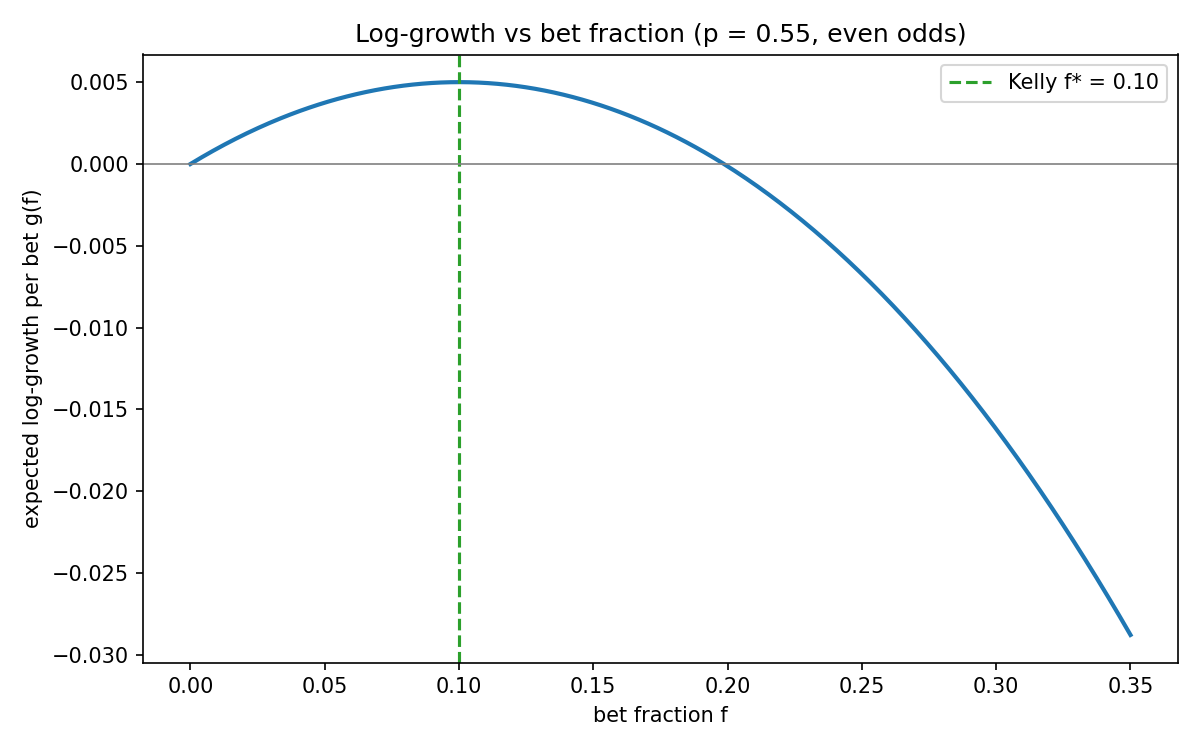
\includegraphics[keepaspectratio]{figures/growth_curve.png}}

}

\caption{Expected log-growth versus bet fraction. The curve is
asymmetric about its peak: over-betting is punished more severely than
under-betting.}

\end{figure}%

\begin{figure}[H]

{\centering \pandocbounded{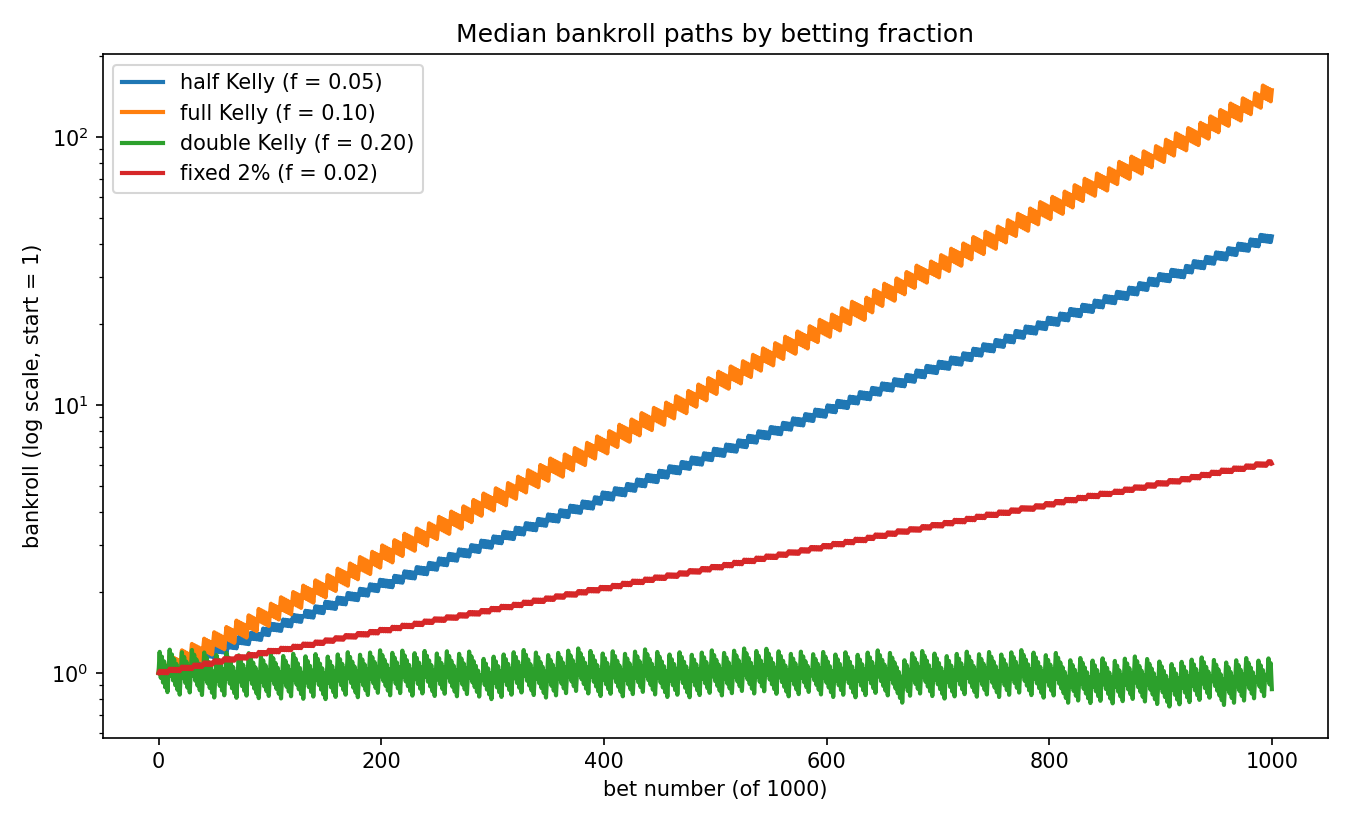
\includegraphics[keepaspectratio]{figures/bankroll_paths.png}}

}

\caption{Median bankroll paths by betting fraction (log scale).}

\end{figure}%

\subsection{Kelly with an estimated
edge}\label{kelly-with-an-estimated-edge}

Real bettors estimate \(p\). The study models a bettor who observes
\(n\) historical outcomes, forms the sample win rate \(\hat p\), and
bets \(m \times f^\*(\hat p)\) --- a \emph{Kelly multiplier} \(m\)
applied to the Kelly fraction of the estimate --- against the true
\(p\).

\textbf{Noise.} Sweeping \(m\) for several history lengths, the
growth-maximising multiplier falls as the estimate degrades:

{\def\LTcaptype{none} % do not increment counter
\begin{longtable}[]{@{}lrr@{}}
\toprule\noalign{}
Estimate quality & Best multiplier & Growth at best \\
\midrule\noalign{}
\endhead
\bottomrule\noalign{}
\endlastfoot
Known edge (theory) & 1.00 & 0.00501 \\
Estimated from 1,000 bets & 0.90 & 0.00459 \\
Estimated from 200 bets & 0.65 & 0.00360 \\
Estimated from 50 bets & 0.45 & 0.00263 \\
\end{longtable}
}

\textbf{Bias.} A bettor who believes \(p = 0.55\) when the truth is
\(0.52\) --- three points of overconfidence, easily produced by backtest
overfitting --- realises \emph{negative} growth (\(-0.0035\) per bet) at
full Kelly on the believed edge, while \(m \approx 0.3\) remains
profitable.

The mechanism is the asymmetry of \(g(f)\) visible in the growth-curve
figure: errors that push \(f\) beyond the peak cost more than equal
errors short of it, so uncertainty shifts the optimum toward
conservatism. This is the quantitative content of the practitioner's
rule ``bet fractional Kelly.''

\begin{figure}[H]

{\centering \pandocbounded{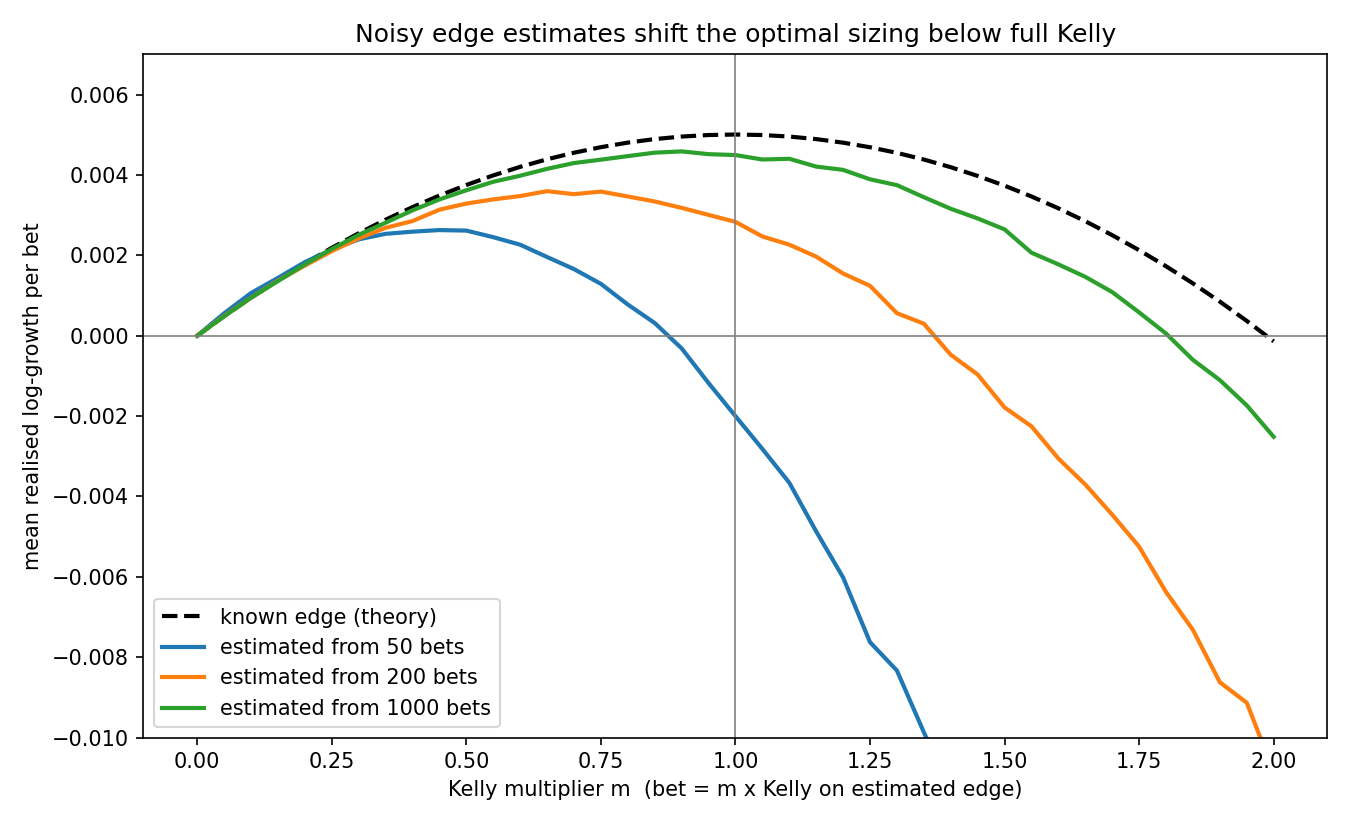
\includegraphics[keepaspectratio]{figures/noisy_edge_multiplier.png}}

}

\caption{Realised growth versus Kelly multiplier under estimation
noise.}

\end{figure}%

\begin{figure}[H]

{\centering \pandocbounded{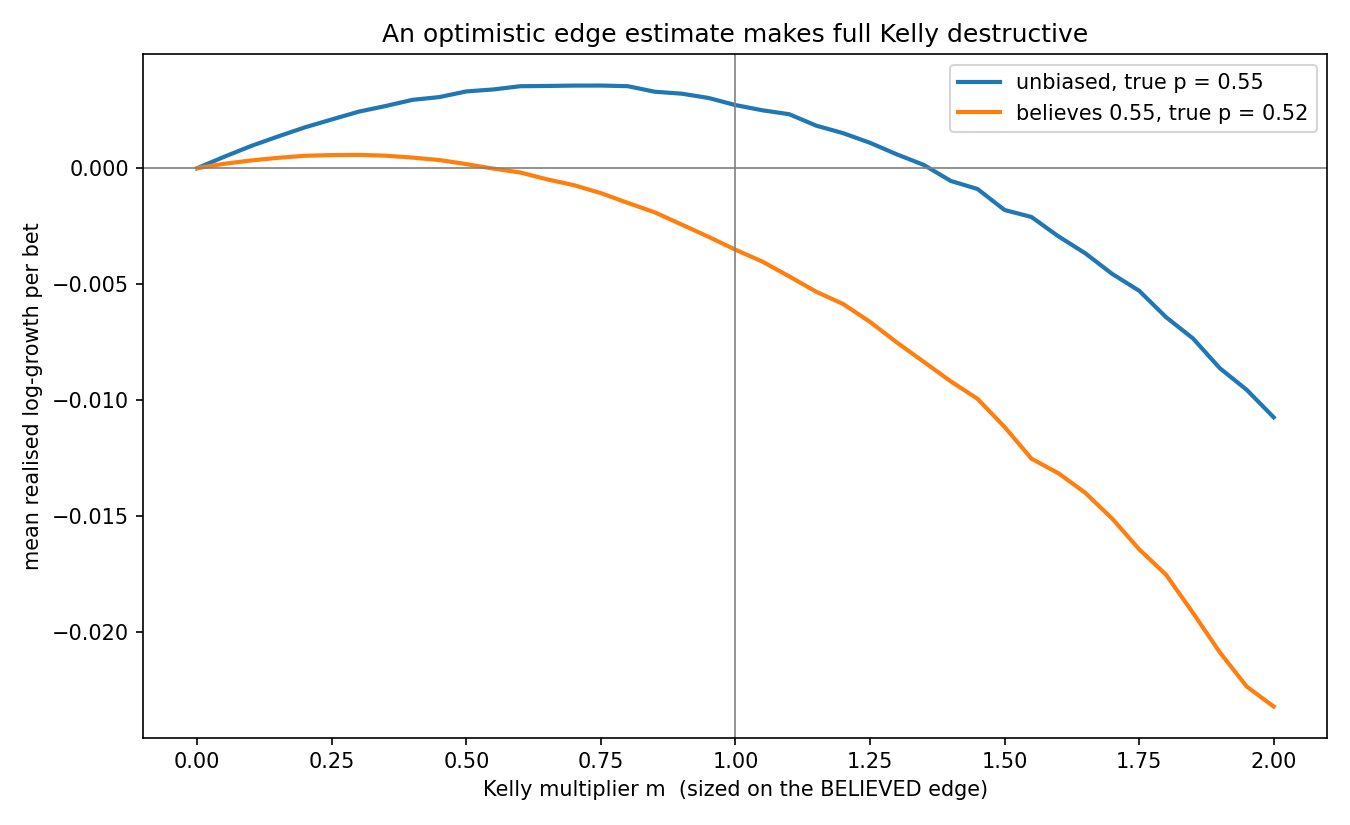
\includegraphics[keepaspectratio]{figures/biased_edge_multiplier.png}}

}

\caption{An optimistic edge estimate makes full Kelly destructive.}

\end{figure}%

\section{Section 2: Market making against informed
flow}\label{section-2-market-making-against-informed-flow}

\subsection{The game}\label{the-game}

A hidden value \(V\) is the sum of three dice (\(V \in \{3,\dots,18\}\),
mean \(10.5\)). Each round a market maker quotes a bid and an ask; one
trader arrives. With probability \(1-\phi\) the trader is a \emph{noise
trader} who buys or sells at random; with probability \(\phi\) they are
\emph{informed}, observing \(V + \varepsilon\) with
\(\varepsilon \sim \mathcal N(0, \sigma^2)\), buying if their signal
exceeds the ask, selling if below the bid, and passing otherwise. All
positions settle at \(V\) after 100 rounds.

The maker's economics decompose cleanly: noise traders pay the
half-spread on every fill regardless of price level (revenue), while
informed traders fill only when the quotes are wrong, transferring the
mispricing to themselves (cost). This selective participation is
\textbf{adverse selection}, and it is asymmetric in a way the simulation
makes vivid: informed traders are absent from the fill stream precisely
when the maker is priced correctly.

\subsection{The cost of not listening}\label{the-cost-of-not-listening}

A naive maker quoting a fixed \(\pm 1.0\) spread around the prior mean,
across 2,000 games:

{\def\LTcaptype{none} % do not increment counter
\begin{longtable}[]{@{}rrrr@{}}
\toprule\noalign{}
Informed share & Mean P\&L & Median P\&L & P(loss) \\
\midrule\noalign{}
\endhead
\bottomrule\noalign{}
\endlastfoot
0\% & 98.4 & 100.0 & 0.005 \\
30\% & 27.7 & 45.5 & 0.255 \\
60\% & \textbf{-48.4} & -24.0 & 0.533 \\
\end{longtable}
}

In the example game plotted below, \(V = 3\) --- far below the prior ---
and informed traders sell into the maker's bid for the entire game while
it never updates. The loss is structural.

\begin{figure}[H]

{\centering \pandocbounded{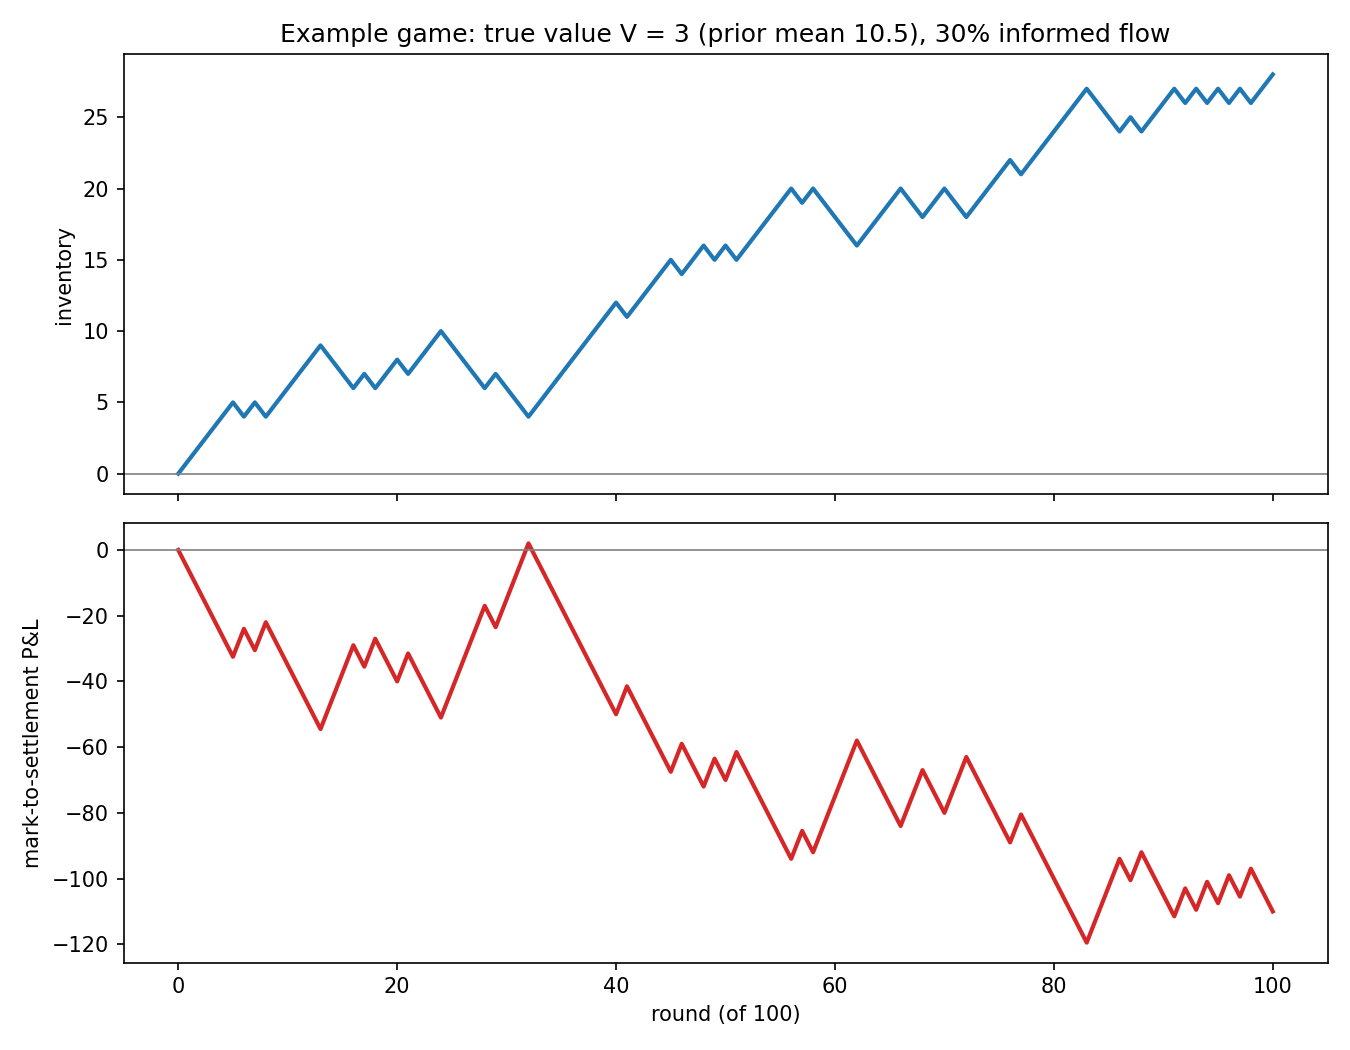
\includegraphics[keepaspectratio]{figures/example_game.png}}

}

\caption{A single game with \(V=3\): the naive maker accumulates a long
position at prices far above value.}

\end{figure}%

\begin{figure}[H]

{\centering \pandocbounded{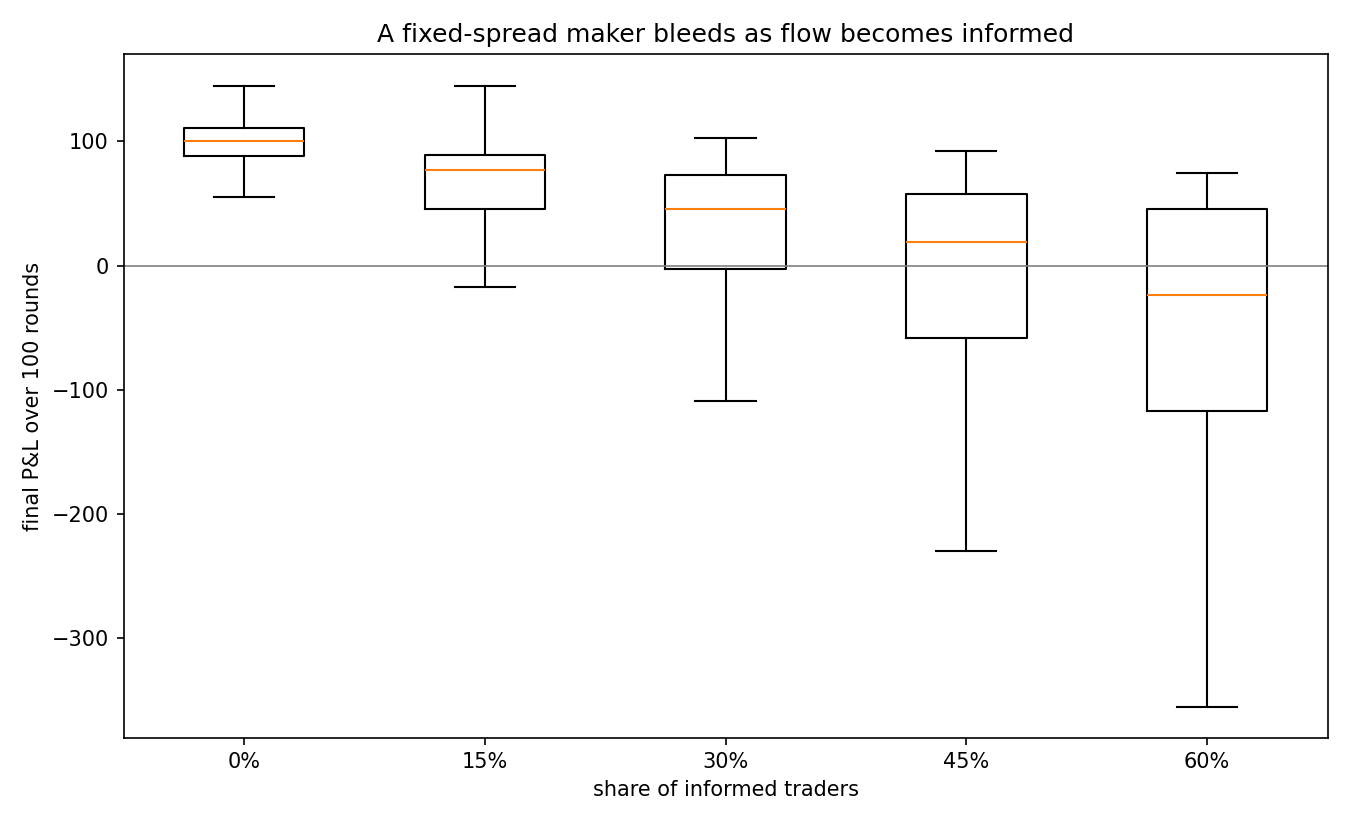
\includegraphics[keepaspectratio]{figures/informed_share_sweep.png}}

}

\caption{Final P\&L distribution versus informed share for the naive
maker.}

\end{figure}%

\subsection{Strategies that listen}\label{strategies-that-listen}

Two upgrades were implemented and raced on identical market conditions:

\begin{itemize}
\tightlist
\item
  \textbf{Inventory-aware}: quote centre \(= 10.5 - \kappa \times\)
  inventory. Position control with no learning.
\item
  \textbf{Bayesian}: a discrete posterior over \(V\), updated after
  \emph{every} event using the game's known structure. The likelihoods
  are, for candidate value \(v\) and quotes
  \((\text{bid}, \text{ask})\):
\end{itemize}

\[
\begin{aligned}
P(\text{buy} \mid v) &= \tfrac{1-\phi}{2} + \phi\,\Pr(v + \varepsilon > \text{ask}) \\
P(\text{sell} \mid v) &= \tfrac{1-\phi}{2} + \phi\,\Pr(v + \varepsilon < \text{bid}) \\
P(\text{pass} \mid v) &= \phi\,\Pr(\text{bid} \le v + \varepsilon \le \text{ask})
\end{aligned}
\]

Noise traders never pass, so a pass is \emph{pure signal} that \(V\)
lies inside the spread --- an observation with no analogue in fill-only
models, and one the convergence figure shows the maker exploiting.

Tournament results (1,500 games per point):

{\def\LTcaptype{none} % do not increment counter
\begin{longtable}[]{@{}rrrr@{}}
\toprule\noalign{}
Informed share & Naive & Inventory-aware & Bayesian \\
\midrule\noalign{}
\endhead
\bottomrule\noalign{}
\endlastfoot
0\% & 98.0 & 98.4 & 98.6 \\
30\% & 27.3 & 60.2 & 68.2 \\
60\% & \textbf{-46.2} & 41.0 & \textbf{48.4} \\
\end{longtable}
}

The same flow that bleeds the naive maker \emph{funds} the Bayesian one
with information.

\begin{figure}[H]

{\centering \pandocbounded{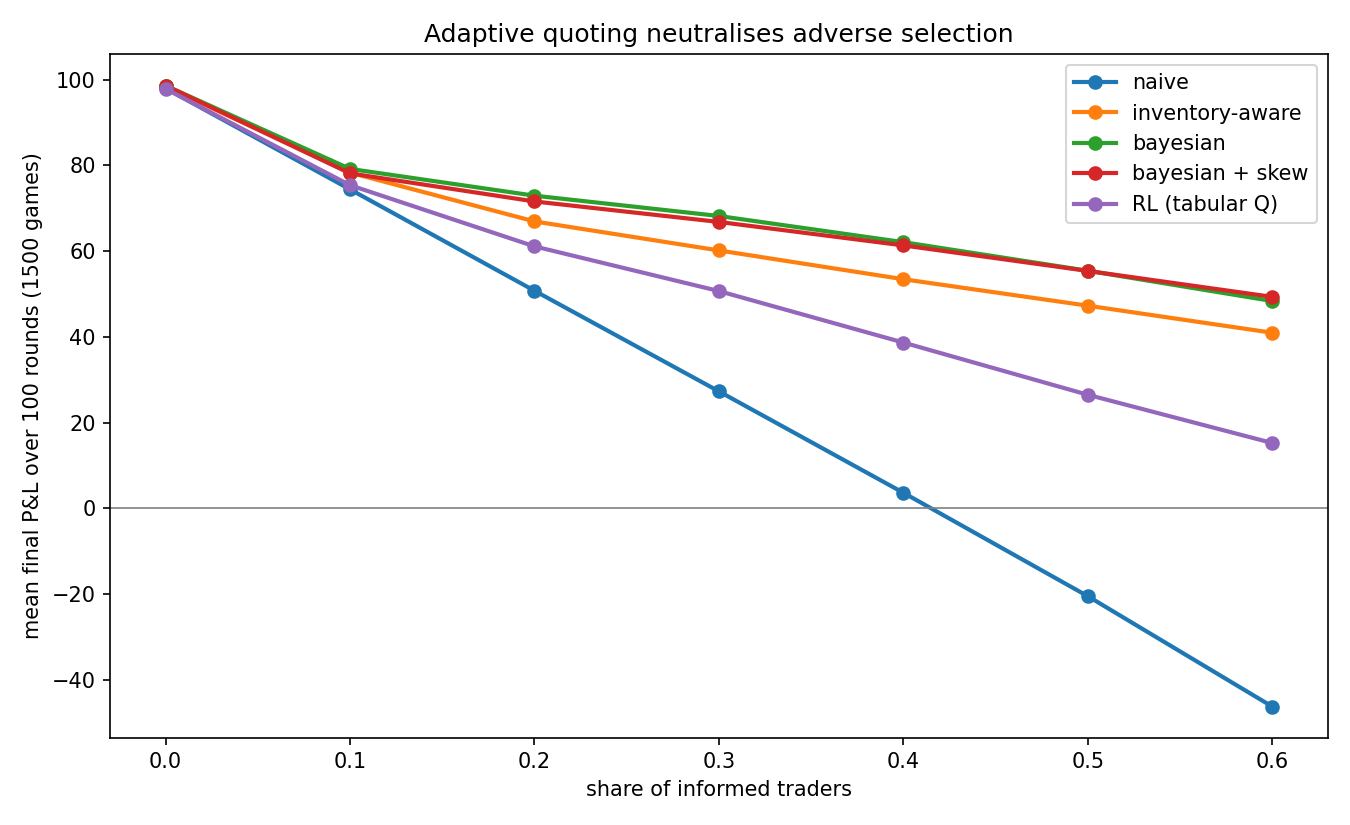
\includegraphics[keepaspectratio]{figures/strategy_tournament.png}}

}

\caption{Strategy tournament: adaptive quoting neutralises adverse
selection.}

\end{figure}%

\begin{figure}[H]

{\centering \pandocbounded{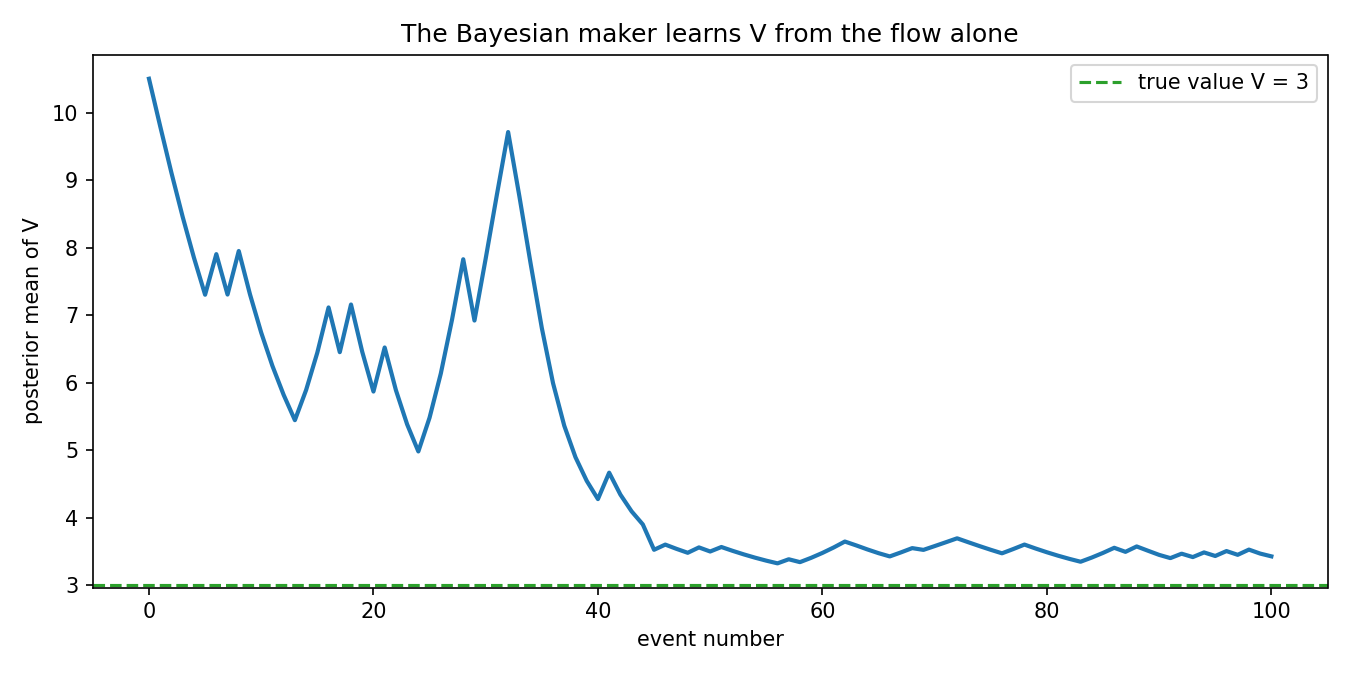
\includegraphics[keepaspectratio]{figures/bayesian_convergence.png}}

}

\caption{The Bayesian maker's posterior mean homing in on \(V=3\) from
the flow alone.}

\end{figure}%

\section{Section 3: A reinforcement-learning market
maker}\label{section-3-a-reinforcement-learning-market-maker}

\subsection{Problem formulation}\label{problem-formulation}

The scientific question: can a model-free agent, denied the game's
structure (\(\phi\), \(\sigma\), even the existence of informed
traders), learn a quoting policy from experience? Because \(V\) is
hidden, the problem is a \textbf{partially observable MDP}; the
theoretically sufficient state is the belief distribution over \(V\),
which is exactly what the Bayesian maker tracks. The agent is instead
given a deliberately crude, hand-crafted summary of history:

\begin{enumerate}
\def\labelenumi{\arabic{enumi}.}
\tightlist
\item
  \textbf{flow imbalance} (buys minus sells so far) --- the human
  player's ``which side keeps getting hit'' signal;
\item
  \textbf{quote-centre offset} from the prior --- without which
  imbalance is uninterpretable, since it cannot be known whether the
  imbalance has already been responded to;
\item
  \textbf{inventory} --- settlement risk;
\item
  \textbf{a coarse game clock} --- early rounds reward information
  gathering, late rounds punish open positions.
\end{enumerate}

Each feature is discretised (bins \(7 \times 7 \times 5 \times 3\)), and
the action space is five discrete quote-centre moves
\(\{-1.0, -0.5, 0, +0.5, +1.0\}\) at a fixed \(\pm 1.0\) spread. The
reward is the per-fill mispricing (\(\text{ask} - V\) on a sale,
\(V - \text{bid}\) on a purchase), which telescopes exactly to the
settled P\&L --- a property pinned by a unit test. \(V\) appears in the
reward \emph{computation} during training but never in the observation:
the standard training-signal/input distinction.

\subsection{Algorithm}\label{algorithm}

Tabular Q-learning {[}Watkins, 1989{]}: maintain \(Q(s,a)\), and after
each transition \((s, a, r, s')\) update

\[
Q(s,a) \leftarrow Q(s,a) + \alpha\left[r + \gamma \max_{a'} Q(s',a') - Q(s,a)\right],
\]

with \(\gamma = 1\) (episodic task, monetary reward),
\(\varepsilon\)-greedy exploration decaying \(1.0 \to 0.05\) over 60\%
of training, and terminal states bootstrapping zero. Q-learning is
off-policy: the update targets the greedy policy's value even while
behaviour is exploratory.

Evaluation discipline was enforced throughout: greedy-policy evaluation
on held-out seed blocks disjoint from training seeds;
\textbf{best-checkpoint selection} (motivated below); and final
reporting on a third seed block untouched by either training or
selection.

\subsection{Results}\label{results}

A first 20,000-episode run with constant \(\alpha = 0.1\) exhibited the
characteristic instability of tabular Q-learning: evaluation oscillated
between \(\approx 48\) and \(\approx 18\), and the final-episode
snapshot happened to score 20.7 --- a bad snapshot of a decent agent.
Halving \(\alpha\) and keeping the best evaluated checkpoint produced a
stable plateau and a final score of \textbf{49.2 over 1,000 fresh
held-out games}, against a hold-still benchmark of \(\approx 29\) and
the Bayesian ceiling of \(\approx 68\): roughly half the
naive-to-Bayesian gap recovered from four coarse features. State
coverage was 29\% of bins; most extreme feature combinations are
unreachable in 100-round games.

\begin{figure}[H]

{\centering \pandocbounded{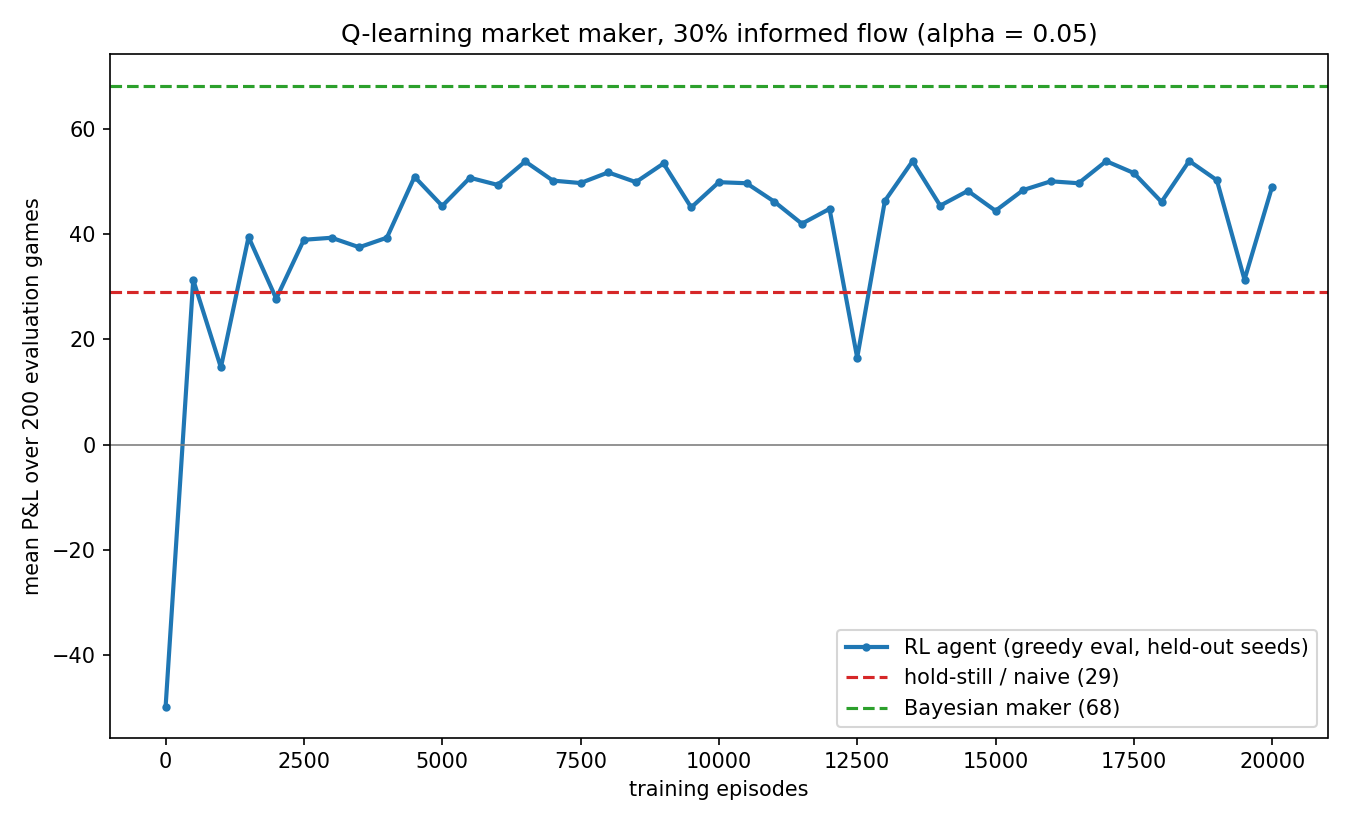
\includegraphics[keepaspectratio]{figures/rl_learning_curve.png}}

}

\caption{Learning curve: evaluation P\&L versus training episodes, with
naive and Bayesian benchmarks.}

\end{figure}%

Entered in the tournament via a thin adapter (the frozen table wrapped
in the MarketMaker interface, reconstructing its observation from its
own fill stream), and noting the agent was trained \emph{only} at
\(\phi = 0.3\):

{\def\LTcaptype{none} % do not increment counter
\begin{longtable}[]{@{}rrrrr@{}}
\toprule\noalign{}
Informed share & Naive & Inventory-aware & Bayesian & RL (tabular Q) \\
\midrule\noalign{}
\endhead
\bottomrule\noalign{}
\endlastfoot
0\% & 98.0 & 98.4 & 98.6 & 97.9 \\
30\% & 27.3 & 60.2 & 68.2 & 50.7 \\
60\% & -46.2 & 41.0 & 48.4 & 15.3 \\
\end{longtable}
}

The agent beats the naive maker everywhere and remains profitable at
60\% informed flow, where the naive maker loses heavily. It does
\textbf{not} overtake the hand-designed inventory-aware heuristic: at
this scale of state space and training budget, a good inductive bias is
hard to out-learn. Its out-of-distribution decay (trained at 30\%,
weaker at the extremes) is visible and expected.

\section{Discussion and limitations}\label{discussion-and-limitations}

Three threads tie the sections together. First, \emph{information
asymmetry has a price and a location}: in the betting studies it appears
as the cost of acting on estimates as if they were truths; in market
making it appears as adverse selection. Second, \emph{the asymmetry of
losses dictates conservatism}: the concavity of log-growth and the
one-sidedness of informed flow both mean errors are not symmetric, so
optimal behaviour backs away from the frictionless optimum. Third,
\emph{listening is worth money}: the gap between the naive and Bayesian
makers, and the RL agent's ability to close half of it from crude
features, are both measurements of the value of information in the order
flow.

Limitations, stated plainly: the game is stationary within an episode
(no news, no drifting \(V\)); trader arrival is one-per-round with unit
size; the Bayesian maker is given the true \(\phi\) and \(\sigma\),
making its benchmark a ceiling rather than a fair competitor; the RL
agent's features are hand-crafted, its discretisation coarse, and it was
trained at a single informed share. The betting studies assume binary
independent bets; correlated simultaneous bets (portfolio Kelly) remain
on the roadmap.

\section{Future work}\label{future-work}

Policy inspection (heatmaps of the learned greedy action over
imbalance-by-centre slices, compared with the Bayesian maker's
behaviour); ablations (sparse versus dense reward; removing the
flow-imbalance feature, which should collapse the agent to inventory
management); a DQN on the identical environment via stable-baselines3,
relaxing the discretisation; an adaptive Bayesian maker that infers
\(\phi\) online; and the portfolio Kelly extension connecting Section 1
to multi-asset allocation.

\section{Reproducibility}\label{reproducibility}

All experiments are seeded scripts in \texttt{scripts/}; all figures in
this document are their direct outputs. The full test suite (40 tests)
runs with \texttt{python\ -m\ pytest}. Code:
\texttt{github.com/jacksonfraser-aero/kelly-betting-simulator}.

\section*{References}\label{references}
\addcontentsline{toc}{section}{References}

\begin{itemize}
\tightlist
\item
  Kelly, J. L. (1956). \emph{A New Interpretation of Information Rate.}
  Bell System Technical Journal.
\item
  Thorp, E. O. (2006). \emph{The Kelly Criterion in Blackjack, Sports
  Betting, and the Stock Market.}
\item
  MacLean, L., Thorp, E. O., \& Ziemba, W. (2011). \emph{The Kelly
  Capital Growth Investment Criterion.} World Scientific.
\item
  Glosten, L., \& Milgrom, P. (1985). \emph{Bid, Ask and Transaction
  Prices in a Specialist Market with Heterogeneously Informed Traders.}
  Journal of Financial Economics.
\item
  Watkins, C. (1989). \emph{Learning from Delayed Rewards.} PhD thesis,
  Cambridge.
\item
  Sutton, R., \& Barto, A. (2018). \emph{Reinforcement Learning: An
  Introduction} (2nd ed.). MIT Press.
\end{itemize}




\end{document}
